%iffalse
\let\negmedspace\undefined
\let\negthickspace\undefined
\documentclass[journal,12pt,onecolumn]{IEEEtran}
\usepackage{cite}
\usepackage{amsmath,amssymb,amsfonts,amsthm}
\usepackage{algorithmic}
\usepackage{graphicx}
\usepackage{textcomp}
\usepackage{xcolor}
\usepackage{txfonts}
\usepackage{listings}
\usepackage{enumitem}
\usepackage{mathtools}
\usepackage{gensymb}
\usepackage{comment}
\usepackage[breaklinks=true]{hyperref}
\usepackage{tkz-euclide} 
\usepackage{gvv}                                        
%\def\inputGnumericTable{}                                 
\usepackage[latin1]{inputenc}     
\usepackage{xparse}
\usepackage{color}                                            
\usepackage{array}                                            
\usepackage{longtable}                                       
\usepackage{calc}                                             
\usepackage{multirow}
\usepackage{multicol}
\usepackage{hhline}                                           
\usepackage{ifthen}                                           
\usepackage{lscape}
\usepackage{tabularx}
\usepackage{array}
\usepackage{float}
\usepackage{circuitikz}
\usepackage{tikz}
\usepackage{pgfplots}
\pgfplotsset{compat=1.18}
\usetikzlibrary{arrows.meta}
\usetikzlibrary{decorations.pathmorphing}
\newtheorem{theorem}{Theorem}[section]
\newtheorem{problem}{Problem}
\newtheorem{proposition}{Proposition}[section]
\newtheorem{lemma}{Lemma}[section]
\newtheorem{corollary}[theorem]{Corollary}
\newtheorem{example}{Example}[section]
\newtheorem{definition}[problem]{Definition}
\newcommand{\BEQA}{\begin{eqnarray}}
\newcommand{\EEQA}{\end{eqnarray}}
\newcommand{\define}{\stackrel{\triangle}{=}}
\theoremstyle{remark}
\newtheorem{rem}{Remark}
% Marks the beginning of the document
\begin{document}
\title{gate 2}
\author{EE24Btech11041 - Mohit}
\maketitle
\renewcommand{\thefigure}{\theenumi}
\renewcommand{\thetable}{\theenumi}


\begin{enumerate}

\item Flow around a Rankine half-body is represented by the superposition of
\hfill{(XE 2014)}
\begin{multicols}{4}
\begin{enumerate}

\item source and vortex flows.
\item source and uniform flows.
\item vortex and uniform flows.
\item source, vortex and uniform flows.

\end{enumerate}
\end{multicols}

\item It is required to carry out model studies on a boat having a characteristic length of $3.6 m$ and travelling at a speed of $3 m/s$. Assume the acceleration due to gravity as $10 m/s^{2}$ and neglect the effects due to viscous and surface tension forces. The value of appropriate non-dimensional number is \rule{2cm}{0.4pt}.

\item Which one of the following velocity profiles typically represents a fully developed incompressible, turbulent flow in a pipe? 

\hfill{(XE 2014)}
\begin{multicols}{4}
\begin{enumerate}

\item 

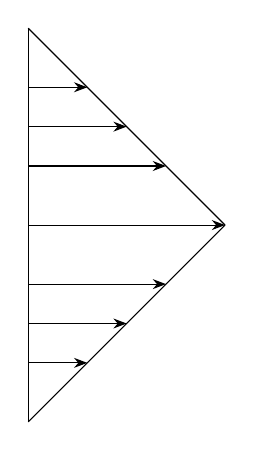
\begin{tikzpicture}
\tikzstyle{every node}=[font=\LARGE]
\draw [short] (11.25,8.5) -- (11.25,3.5);
\draw [short] (11.25,8.5) -- (13.75,6);
\draw [short] (11.25,3.5) -- (13.75,6);
\draw [->, >=Stealth] (11.25,6) -- (13.75,6);
\draw [->, >=Stealth] (11.25,6.75) -- (13,6.75);
\draw [->, >=Stealth] (11.25,5.25) -- (13,5.25);
\draw [->, >=Stealth] (11.25,7.25) -- (12.5,7.25);
\draw [->, >=Stealth] (11.25,4.75) -- (12.5,4.75);
\draw [->, >=Stealth] (11.25,7.75) -- (12,7.75);
\draw [->, >=Stealth] (11.25,4.25) -- (12,4.25);
\end{tikzpicture}

\item 
{\scalebox{0.22}{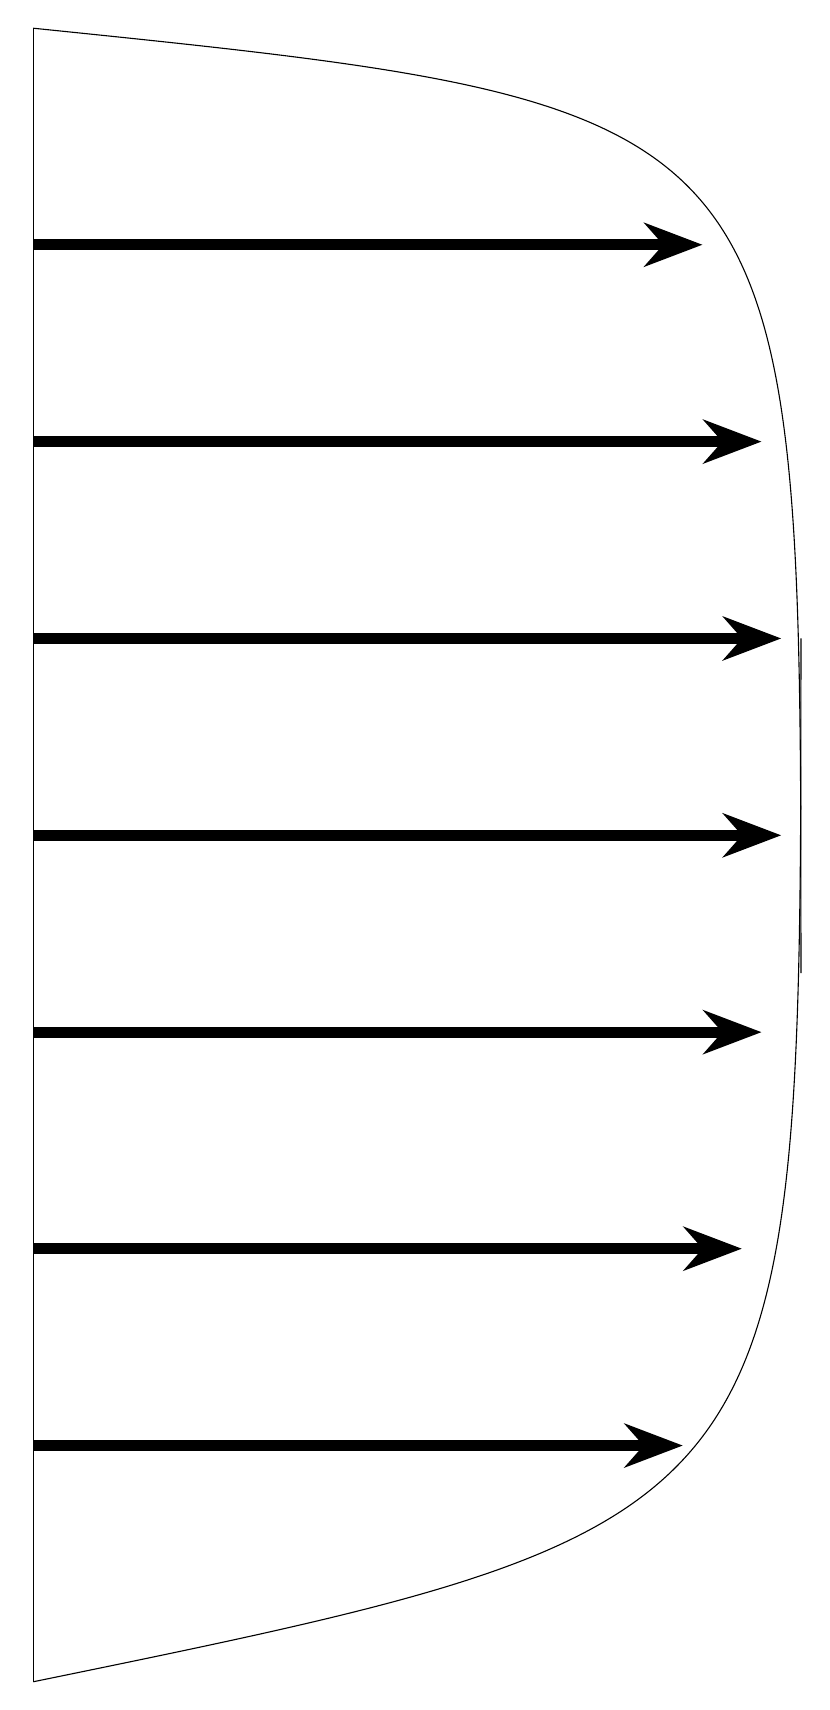
\begin{tikzpicture}
\tikzstyle{every node}=[font=\LARGE]
\draw [short] (14.75,13.75) .. controls (24.5,12.75) and (24.5,12.75) .. (24.5,1.75);
\draw [short] (14.75,-7.25) .. controls (24.5,-5.25) and (24.5,-5.25) .. (24.5,6);
\draw [short] (14.75,13.75) -- (14.75,-7.25);
\draw [line width=4pt,->, >=Stealth] (14.75,11) -- (23.25,11);
\draw [line width=4pt,->, >=Stealth] (14.75,8.5) -- (24,8.5);
\draw [line width=4pt,->, >=Stealth] (14.75,6) -- (24.25,6);
\draw [line width=4pt,->, >=Stealth] (14.75,3.5) -- (24.25,3.5);
\draw [line width=4pt,->, >=Stealth] (14.75,1) -- (24,1);
\draw [line width=4pt,->, >=Stealth] (14.75,-1.75) -- (23.75,-1.75);
\draw [line width=4pt,->, >=Stealth] (14.75,-4.25) -- (23,-4.25);
\end{tikzpicture}
}
}

\item 
{\scalebox{0.6}{\begin{tikzpicture}
\tikzstyle{every node}=[font=\LARGE]
\draw [short] (9.5,15.25) .. controls (13.25,11.25) and (13.25,11.25) .. (9.5,7);
\draw [short] (9.5,15.25) -- (9.5,7);
\draw [->, >=Stealth] (9.5,11) -- (12.25,11);
\draw [->, >=Stealth] (9.5,11.75) -- (12.25,11.75);
\draw [->, >=Stealth] (9.5,12.5) -- (11.75,12.5);
\draw [->, >=Stealth] (9.5,13.25) -- (11.25,13.25);
\draw [->, >=Stealth] (9.5,14) -- (10.5,14);
\draw [->, >=Stealth] (9.5,10.25) -- (12,10.25);
\draw [->, >=Stealth] (9.5,9.5) -- (11.5,9.5);
\draw [->, >=Stealth] (9.5,8.75) -- (11,8.75);
\draw [->, >=Stealth] (9.5,8) -- (10.25,8);
\end{tikzpicture}
}
}


\item 
{\scalebox{0.9}{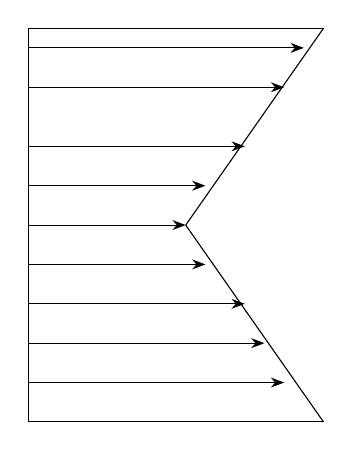
\begin{tikzpicture}
\tikzstyle{every node}=[font=\LARGE]
\draw [short] (7.5,16) -- (7.5,11);
\draw [short] (7.5,16) -- (11.25,16);
\draw [short] (9.5,13.5) -- (11.25,16);
\draw [short] (9.5,13.5) -- (11.25,11);
\draw [short] (7.5,11) -- (11.25,11);
\draw [->, >=Stealth] (7.5,13.5) -- (9.5,13.5);
\draw [->, >=Stealth] (7.5,14) -- (9.75,14);
\draw [->, >=Stealth] (7.5,14.5) -- (10.25,14.5);
\draw [->, >=Stealth] (7.5,15.25) -- (10.75,15.25);
\draw [->, >=Stealth] (7.5,15.75) -- (11,15.75);
\draw [->, >=Stealth] (7.5,13) -- (9.75,13);
\draw [->, >=Stealth] (7.5,12.5) -- (10.25,12.5);
\draw [->, >=Stealth] (7.5,12) -- (10.5,12);
\draw [->, >=Stealth] (7.5,11.5) -- (10.75,11.5);
\end{tikzpicture}
}
}

\end{enumerate}
\end{multicols}

\item Consider an incompressible, laminar flow past a circular cylinder of diameter d. The flow is uniform at the far upstream. Which one of the following figures typically represents the wake velocity profile just downstream of the cylinder?
 
\hfill{(XE 2014)}
\begin{multicols}{2}
\begin{enumerate}

\item
 {\scalebox{0.4}{\begin{tikzpicture}
\tikzstyle{every node}=[font=\LARGE]
\draw [->, >=Stealth] (11.25,12.25) -- (16.25,12.25);
\draw [->, >=Stealth] (11.25,11) -- (16.25,11);
\draw [->, >=Stealth] (11.25,9.75) -- (16.25,9.75);
\draw [->, >=Stealth] (11.25,8.5) -- (16.25,8.5);
\draw [->, >=Stealth] (11.25,7.25) -- (16.25,7.25);
\draw [->, >=Stealth] (11.25,6) -- (16.25,6);
\draw [->, >=Stealth] (11.25,4.75) -- (16.25,4.75);
\draw [->, >=Stealth] (23.75,12.25) -- (28.75,12.25);
\draw [->, >=Stealth] (23.75,4.75) -- (28.75,4.75);
\draw [->, >=Stealth] (23.75,6) -- (27.75,6);
\draw [->, >=Stealth] (23.75,11) -- (27.75,11);
\node [font=\LARGE] at (19.5,8.5) {d};
\draw [->, >=Stealth] (23.75,9.75) -- (26.75,9.75);
\draw [->, >=Stealth] (23.75,7.25) -- (26.75,7.25);
\draw [->, >=Stealth] (23.75,8.5) -- (25.75,8.5);
\draw [short] (11.25,12.25) -- (11.25,4.75);
\draw [short] (16.25,12.25) -- (16.25,4.5);
\draw [short] (28.75,12.25) -- (25.75,8.5);
\draw  (20,8.5) circle (1.75cm);
\draw [<->, >=Stealth] (20,10.25) -- (20,6.75);
\draw [short] (23.75,12.25) -- (23.75,4.75);
\draw [short] (28.75,4.75) -- (25.75,8.5);
\end{tikzpicture}
}
}

\item 
{\scalebox{0.4}{\begin{circuitikz}
\tikzstyle{every node}=[font=\LARGE]
\draw [->, >=Stealth] (11.25,12.25) -- (16.25,12.25);
\draw [->, >=Stealth] (11.25,11) -- (16.25,11);
\draw [->, >=Stealth] (11.25,9.75) -- (16.25,9.75);
\draw [->, >=Stealth] (11.25,8.5) -- (16.25,8.5);
\draw [->, >=Stealth] (11.25,7.25) -- (16.25,7.25);
\draw [->, >=Stealth] (11.25,6) -- (16.25,6);
\draw [->, >=Stealth] (11.25,4.75) -- (16.25,4.75);
\draw [short] (11.25,12.25) -- (11.25,4.75);
\draw [short] (16.25,12.25) -- (16.25,4.5);
\draw  (20,8.5) circle (1.75cm);
\draw [<->, >=Stealth] (20,10.25) -- (20,6.75);
\node [font=\LARGE] at (19.5,8.5) {d};
\begin{scope}[rotate around={-90:(26.25,12.25)}]
\draw[domain=26.25:33.75,samples=100,smooth] plot (\x,{1.5*sin(0.9*\x r -22.0 r ) +12.25});
\end{scope}
\draw [short] (26.25,12.25) -- (26.25,4.75);
\draw [->, >=Stealth] (26.25,12.25) -- (27.75,12.25);
\draw [->, >=Stealth] (26.25,11.5) -- (27.25,11.5);
\draw [->, >=Stealth] (26.25,9.5) -- (25.0,9.5);
\draw [->, >=Stealth] (26.25,8.5) -- (24.75,8.5);
\draw [->, >=Stealth] (26.25,7.75) -- (25.25,7.75);
\draw [->, >=Stealth] (26.25,5.75) -- (27.75,5.75);
\draw [->, >=Stealth] (26.25,4.75) -- (27.5,4.75);
\end{circuitikz} 
}
}


\item 
{\scalebox{0.4}{\begin{tikzpicture}
\tikzstyle{every node}=[font=\LARGE]
\draw [->, >=Stealth] (11.25,12.25) -- (16.25,12.25);
\draw [->, >=Stealth] (11.25,11) -- (16.25,11);
\draw [->, >=Stealth] (11.25,9.75) -- (16.25,9.75);
\draw [->, >=Stealth] (11.25,8.5) -- (16.25,8.5);
\draw [->, >=Stealth] (11.25,7.25) -- (16.25,7.25);
\draw [->, >=Stealth] (11.25,6) -- (16.25,6);
\draw [->, >=Stealth] (11.25,4.75) -- (16.25,4.75);
\draw [short] (11.25,12.25) -- (11.25,4.75);
\draw [short] (16.25,12.25) -- (16.25,4.5);
\draw  (20,8.5) circle (1.75cm);
\draw [<->, >=Stealth] (20,10.25) -- (20,6.75);
\node [font=\LARGE] at (19.5,8.5) {d};
\begin{scope}[rotate around={-90:(25,12.25)}]
\draw[domain=25:32.5,samples=100,smooth] plot (\x,{1.5*sin(0.89*\x r -23.75 r ) +12.25});
\end{scope}
\draw [short] (25,12.25) -- (25,4.75);
\draw [->, >=Stealth] (25,12.25) -- (23.5,12.25);
\draw [->, >=Stealth] (25,11.5) -- (23.75,11.5);
\draw [->, >=Stealth] (25,9.5) -- (26.25,9.5);
\draw [->, >=Stealth] (25,8.75) -- (26.5,8.75);
\draw [->, >=Stealth] (25,8) -- (26.25,8);
\draw [->, >=Stealth] (25,5.75) -- (23.75,5.75);
\draw [->, >=Stealth] (25,5) -- (23.5,5);
\end{tikzpicture}
}
}

\item 
{\scalebox{0.4}{\begin{tikzpicture}
\tikzstyle{every node}=[font=\LARGE]
\draw [->, >=Stealth] (11.25,12.25) -- (16.25,12.25);
\draw [->, >=Stealth] (11.25,11) -- (16.25,11);
\draw [->, >=Stealth] (11.25,9.75) -- (16.25,9.75);
\draw [->, >=Stealth] (11.25,8.5) -- (16.25,8.5);
\draw [->, >=Stealth] (11.25,7.25) -- (16.25,7.25);
\draw [->, >=Stealth] (11.25,6) -- (16.25,6);
\draw [->, >=Stealth] (11.25,4.75) -- (16.25,4.75);
\draw [short] (11.25,12.25) -- (11.25,4.75);
\draw [short] (16.25,12.25) -- (16.25,4.5);
\draw  (20,8.5) circle (1.75cm);
\draw [<->, >=Stealth] (20,10.25) -- (20,6.75);
\node [font=\LARGE] at (19.5,8.5) {d};
\draw [short] (23.75,12.25) -- (23.75,4.75);
\draw [short] (25,12.25) -- (27.5,8.5);
\draw [short] (25,4.75) -- (27.5,8.5);
\draw [->, >=Stealth] (23.75,12.25) -- (25,12.25);
\draw [->, >=Stealth] (23.75,11) -- (25.75,11);
\draw [->, >=Stealth] (23.75,9.75) -- (26.5,9.75);
\draw [->, >=Stealth] (23.75,8.5) -- (27.25,8.5);
\draw [->, >=Stealth] (23.75,7.25) -- (26.5,7.25);
\draw [->, >=Stealth] (23.75,6) -- (25.5,6);
\draw [->, >=Stealth] (23.75,4.75) -- (25,4.75);
\end{tikzpicture}
}
}

\end{enumerate}
\end{multicols}

\item A container of square cross-section is partially filled with a liquid of density $\rho_1$. The cylinder is intended to float in another liquid of density $\rho_2$, as shown in the figure. The distance between metacentre and centre of buoyancy is $\frac{1}{V_{sub}}$, where $I$ and $V_{sub}$ are area moment of inertia of the cross-section and submerged volume, respectively. Neglect the weight of the container.

\begin{center}
{\scalebox{0.4}{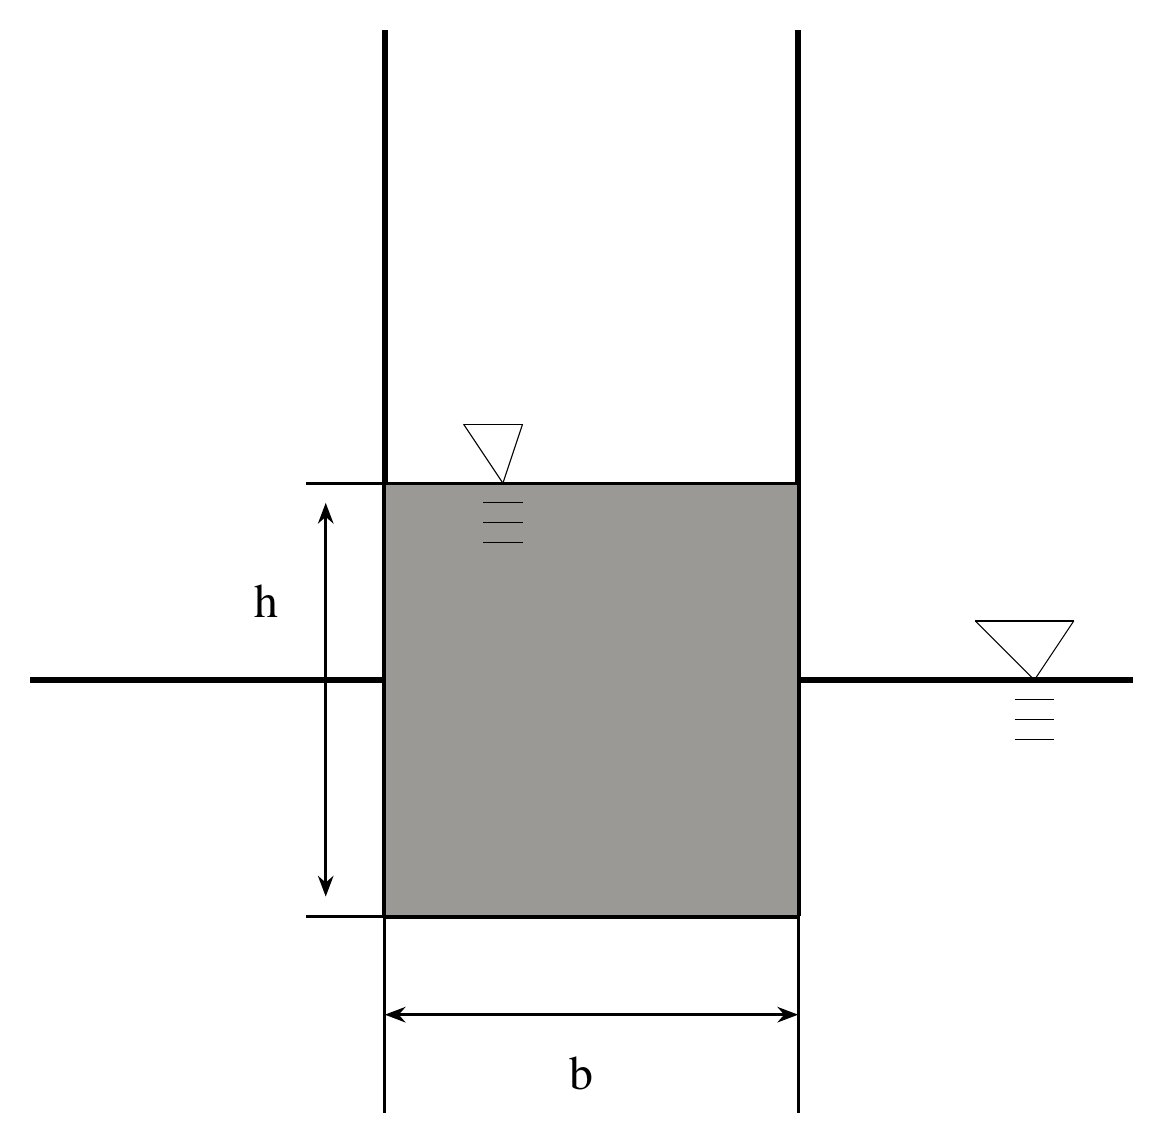
\begin{tikzpicture}
\tikzstyle{every node}=[font=\LARGE]
\draw [line width=2pt, short] (5,19.75) -- (5,8.5);
\draw [line width=2pt, short] (5,8.5) -- (10.25,8.5);
\draw [line width=2pt, short] (10.25,8.5) -- (10,8.5);
\draw [line width=2pt, short] (10.25,8.5) -- (10.25,19.75);
\draw [line width=2pt, short] (10.25,11.5) -- (14.5,11.5);
\draw [line width=2pt, short] (5,11.5) -- (0.5,11.5);
\draw [line width=1pt, short] (5,8.5) -- (5,6);
\draw [line width=1pt, short] (10.25,8.5) -- (10.25,6);
\draw [line width=1pt, short] (4,14) -- (5,14);
\draw [line width=1pt, short] (4,8.5) -- (5,8.5);
\draw [line width=1pt, <->, >=Stealth] (5,7.25) -- (10.25,7.25);
\draw [line width=1pt, <->, >=Stealth] (4.25,13.75) -- (4.25,8.75);
\node [font=\LARGE] at (3.5,12.5) {h};
\node [font=\LARGE] at (7.5,6.5) {b};
\draw [ fill={rgb,255:red,154; green,153; blue,150} , line width=1pt ] (5,14) rectangle (10.25,8.5);
\draw [short] (6,14.75) -- (6.75,14.75);
\draw [short] (6,14.75) -- (6.5,14);
\draw [short] (6.75,14.75) -- (6.5,14);
\draw [short] (12.5,12.25) -- (13.25,11.5);
\draw [short] (13.75,12.25) -- (13.25,11.5);
\draw [short] (12.5,12.25) -- (13.75,12.25);
\draw [short] (13,11.25) -- (13.5,11.25);
\draw [short] (13,11) -- (13.5,11);
\draw [short] (13.25,10.75) -- (13,10.75);
\draw [short] (13,10.75) -- (13.5,10.75);
\draw [short] (6.25,13.75) -- (6.75,13.75);
\draw [short] (6.25,13.5) -- (6.75,13.5);
\draw [short] (6.25,13.25) -- (6.75,13.25);
\end{tikzpicture}
}
}
\end{center}
Which one of the following is the correct condition for stability?

\hfill{(XE 2014)}
\begin{multicols}{2}
\begin{enumerate}


    \item $\frac{\rho_2}{6 \rho_1} \frac{b}{h} - \frac{h}{b} \left( 1 - \frac{\rho_1}{\rho_2} \right) > 0$
    \item $\frac{\rho_2}{6 \rho_1} \frac{b}{h} - \frac{h}{b} \left( 1 + \frac{\rho_1}{\rho_2} \right) > 0$
    \item $\frac{\rho_2}{6 \rho_1} \frac{b}{h} + \frac{h}{b} \left( 1 - \frac{\rho_1}{\rho_2} \right) > 0$
    \item $\frac{\rho_2}{6 \rho_1} \frac{b}{h} + \frac{h}{b} \left( 1 + \frac{\rho_1}{\rho_2} \right) > 0$

\end{enumerate}
\end{multicols}

\item In a steady state two-dimensional potential flow field due to a point source, the acceleration of a
particle at a distance r from the point source is

\hfill{(XE 2014)}
\begin{multicols}{4}
\begin{enumerate}

\item proportional to $r^{-1}$ .
\item proportional to r .
\item a constant
\item proportional to $r^{-3}$ .

\end{enumerate}
\end{multicols}


\item Velocity in a two-dimensional flow at time $t$ and location $\brak{x,y}$ is described as:
$\vec{V}=3t^{2}\hat{i}+(x-1)\hat{j}$. The equation for the path line of a particle passing through the point $\brak{1,0}$ at

\hfill{(XE 2014)}
\begin{multicols}{4}
\begin{enumerate}

\item $x^{4}$-$4y^{3}$
\item $(x-1)^{3}$-$2y^{4}$
\item $(x-1)^{4}$-$64y^{3}$
\item $(x+1)^{4}$-$16y^{3}$

\end{enumerate}
\end{multicols}



\item The gravity driven flow over a hump of height $h$ n a canal is shown in the figure. The height of
the free surface from the canal bed at upstream of the hump is $H$.The free surface height reduces
to $H_1$ above the hump.

\begin{center}
{\scalebox{0.4}{
\begin{circuitikz}
\tikzstyle{every node}=[font=\LARGE]
\draw [ fill={rgb,255:red,26; green,95; blue,180} ] (2.5,7.25) rectangle (17.5,7.75);
\draw [short] (11.25,7.75) .. controls (13.75,9.75) and (13.75,9.75) .. (16.25,7.75);
\draw [short] (2.5,12.25) -- (10.25,12.25);
\draw [short] (10.75,12.25) .. controls (14,11.5) and (14,11.5) .. (17,12.25);
\draw [short] (10.75,12.25) -- (10.25,12.25);
\draw [short] (17.5,12.25) -- (17,12.25);
\draw [<->, >=Stealth] (13.75,11.5) -- (13.75,9.25);
\draw [<->, >=Stealth] (8.75,12) -- (8.75,7.75);
\draw [->, >=Stealth] (3.75,12) -- (5.75,12);
\draw [->, >=Stealth] (3.75,11.5) -- (5.75,11.5);
\draw [->, >=Stealth] (3.75,10.75) -- (5.75,10.75);
\draw [->, >=Stealth] (3.75,10.25) -- (5.75,10.25);
\draw [->, >=Stealth] (3.75,9.5) -- (5.75,9.5);
\draw [->, >=Stealth] (3.75,9) -- (5.75,9);
\draw [->, >=Stealth] (3.75,8.5) -- (5.75,8.5);
\draw [->, >=Stealth] (3.75,8) -- (5.75,8);
\draw [->, >=Stealth] (16.75,10.5) -- (16.75,9.25);
\draw [->, >=Stealth] (16.75,6) -- (16.75,7.75);
\draw [short] (16.25,9.25) -- (17.5,9.25);
\node [font=\LARGE] at (16.75,8.5) {h};
\node [font=\LARGE] at (9.25,10.25) {H};
\draw [short] (2.5,13) -- (3,12.25);
\draw [short] (3.25,13) -- (3,12.25);
\draw [short] (2.5,13) -- (3.25,13);
\draw [short] (2.75,12) -- (3.25,12);
\draw [short] (2.75,11.75) -- (3.25,11.75);
\draw [short] (3,11.5) -- (3.25,11.5);
\node [font=\LARGE] at (14.25,10.25) {$H_1$};
\end{circuitikz}
}
}
\end{center}


Assuming the canal bed to be horizontal, the discharge per unit width is given by

\hfill{(XE 2014)}
\begin{multicols}{4}
\begin{enumerate}

\item $\sqrt{\frac{2g(H - H_1 - h)}{\frac{1}{H_1^2} - \frac{1}{H^2}}}$
    \item $\sqrt{\frac{2gh}{\frac{1}{(H_1 + h)^2} - \frac{1}{H^2}}}$
    \item $\sqrt{\frac{2g(H - H_1)}{\frac{1}{(H_1 + h)^2} - \frac{1}{H^2}}}$
    \item $\sqrt{\frac{2g(H - H_1)}{\frac{1}{H_1^2} - \frac{1}{H^2}}}$
\end{enumerate}
\end{multicols}


\item Steady state incompressible flow through a pipe network is shown in the figure. Inlets marked as $\brak{1}$,$ \brak{2}$, and $\brak{3}$ and exit marked as $\brak{4}$ are shown with their respective diameters. The exit flow rate at $\brak{4}$ is $0.1m^{3}/s$. A $ 20 \% $ increase in flow rate through $\brak{1}$ results in a $10\%$ increase in flow rate through \brak{4}. The original velocity through inlet \brak{3} is \rule{2cm}{0.4pt}$m/s$. 
\hfill{(XE 2014)}

\begin{center}
{\scalebox{0.4}{
\begin{circuitikz}
\tikzstyle{every node}=[font=\LARGE]
\draw [line width=1pt, short] (3.75,17.25) -- (10,17.25);
\draw [line width=1pt, short] (3.75,14.75) -- (10,14.75);
\draw [line width=1pt, short] (3.75,17.25) -- (-2.5,22.25);
\draw [line width=1pt, short] (3.75,14.75) -- (-2.5,9.75);
\draw [line width=1pt, short] (-4.25,16.75) -- (2,16.75);
\draw [line width=1pt, short] (-4.25,15.75) -- (2,15.75);
\draw [line width=1pt, short] (2,16.75) -- (-3.5,21);
\draw [line width=1pt, short] (2,15.75) -- (-3.75,11.5);
\draw [line width=1pt, <->, >=Stealth] (-1.75,19.75) -- (-0.75,20.75);
\draw [line width=1pt, <->, >=Stealth] (-2.5,16.75) -- (-2.5,15.75);
\draw [line width=1pt, <->, >=Stealth] (-2.25,12.5) -- (-1,11.25);
\draw [line width=1.4pt, ->, >=Stealth] (-5.25,23.5) -- (-3.25,21.75);
\draw [line width=1.4pt, ->, >=Stealth] (-7.25,16.25) -- (-4.5,16.25);
\draw [line width=1.4pt, ->, >=Stealth] (-5.25,9.25) -- (-3.25,10.75);
\node [font=\LARGE] at (-4.75,24.25) {(3)};
\node [font=\LARGE] at (-5.5,17.25) {(2)};
\node [font=\LARGE] at (-5,10.75) {(1)};
\node [font=\LARGE, rotate around={-45:(0,0)}] at (-0.5,19.75) {6 cm};
\node [font=\LARGE] at (-1.5,16.25) {5 cm};
\node [font=\LARGE, rotate around={45:(0,0)}] at (-0.75,12.5) {4 cm};
\draw [line width=1.4pt, ->, >=Stealth] (9.75,16) -- (12,16);
\draw [line width=1.4pt, <->, >=Stealth] (5,17) -- (5,14.75);
\node [font=\LARGE] at (6,15.75) {10 cm};
\node [font=\LARGE] at (11.25,17) {(4)};
\end{circuitikz}
}
}
\end{center}

\item A reducing elbow is used to deflect water upward by $30^{\circ}$ as shown in the figure. The mass flow rate at the inlet is $14 kg/s$. Water is entering at a gauge pressure of $200 kPa$ and exits to the atmosphere. The cross-sectional area is $113 cm^{2}$ at the inlet and $7 cm^{2}$ at the exit. Density of water and acceleration due to gravity are $1000 kg/m^{3}$ and $10 m/s^{2}$, respectively. Magnitude of $x$ - component of the water force on the elbow is \_\_\_\_ $N$. 
\hfill{(XE 2014)}
\item A source with a strength of $k_1$ and a vortex with a strength of $ k_2$ are located at the origin.The
resultant velocity at a radial distance $r$ rom the origin due to the superpositon of the source and vortex is expressed as 


\hfill{(XE 2014)}
\begin{multicols}{4}
\begin{enumerate}

\item $\frac{k_1 + k_2}{r}$
\item $\frac{\sqrt{{k_1}^2 + {k_2}^2}}{r}$
\item a constant
\item proportional to $r^{-3}$ .

\end{enumerate}
\end{multicols}

\item Velocity potential for an incompressible fluid flow is given as: $ \phi = 2(x^2 + 2y - y^2)$.Assume the 
value of stream function at the origin to be zero .The value of stream function at $[\brak{x,y} \equiv \brak{2,2}]$ is \rule{2cm}{0.4pt} .
\hfill{(XE 2014)}

\item The model of a conduit is scaled to $\frac{1}{100}$ of the actual size. Seawater is used in the prototype and fresh water is used in the model. Velocity in the prototype is $0.5 m/s$. Density and dynamic viscosity of the seawater are $1025 kg/m^3$ and $1.07 \times 10^{-3} kg/m-s$, respectively. Density and dynamic viscosity of fresh water are $1000 kg/m^{3}$ and $1 \times 10^{-3} kg/m-s$, respectively. Assume the viscous forces to be dominant. The velocity to be maintained in the model to ensure dynamic similarity is \rule{2cm}{0.4pt} $m/s$. 
\hfill{(XE 2014)}
\end{enumerate}
\end{document}
